\begin{IEEEbiography}[{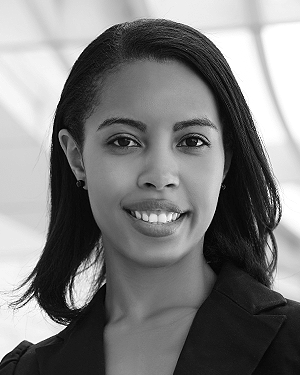
\includegraphics[width=1in,height=1.25in,clip,keepaspectratio]{a1.png}}]{First A. Author} (M'76--SM'81--F'87) and all authors may include
    biographies. Biographies are often not included in conference-related
    papers. This author became a Member (M) of IEEE in 1976, a Senior
    Member (SM) in 1981, and a Fellow (F) in 1987. The first paragraph may
    contain a place and/or date of birth (list place, then date). Next,
    the author's educational background is listed. The degrees should be
    listed with type of degree in what field, which institution, city,
    state, and country, and year the degree was earned. The author's major
    field of study should be lower-cased.

    The second paragraph uses the pronoun of the person (he or she) and not the
    author's last name. It lists military and work experience, including summer
    and fellowship jobs. Job titles are capitalized. The current job must have a
    location; previous positions may be listed
    without one. Information concerning previous publications may be included.
    Try not to list more than three books or published articles. The format for
    listing publishers of a book within the biography is: title of book
    (publisher name, year) similar to a reference. Current and previous research
    interests end the paragraph. The third paragraph begins with the author's
    title and last name (e.g., Dr.\ Smith, Prof.\ Jones, Mr.\ Kajor, Ms.\ Hunter).
    List any memberships in professional societies other than the IEEE. Finally,
    list any awards and work for IEEE committees and publications. If a
    photograph is provided, it should be of good quality, and
    professional-looking. Following are two examples of an author's biography.
\end{IEEEbiography}

\begin{IEEEbiography}[{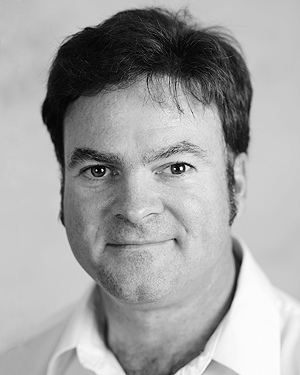
\includegraphics[width=1in,height=1.25in,clip,keepaspectratio]{a2.png}}]{Second B. Author} was born in Greenwich Village, New York, NY, USA in
    1977. He received the B.S. and M.S. degrees in aerospace engineering from
    the University of Virginia, Charlottesville, in 2001 and the Ph.D. degree in
    mechanical engineering from Drexel University, Philadelphia, PA, in 2008.

    From 2001 to 2004, he was a Research Assistant with the Princeton Plasma
    Physics Laboratory. Since 2009, he has been an Assistant Professor with the
    Mechanical Engineering Department, Texas A{\&}M University, College Station.
    He is the author of three books, more than 150 articles, and more than 70
    inventions. His research interests include high-pressure and high-density
    nonthermal plasma discharge processes and applications, microscale plasma
    discharges, discharges in liquids, spectroscopic diagnostics, plasma
    propulsion, and innovation plasma applications. He is an Associate Editor of
    the journal \emph{Earth, Moon, Planets}, and holds two patents.

    Dr. Author was a recipient of the International Association of Geomagnetism
    and Aeronomy Young Scientist Award for Excellence in 2008, and the IEEE
    Electromagnetic Compatibility Society Best Symposium Paper Award in 2011.
\end{IEEEbiography}

\begin{IEEEbiography}[{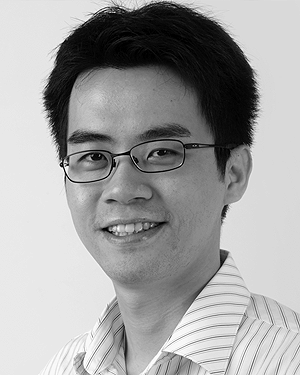
\includegraphics[width=1in,height=1.25in,clip,keepaspectratio]{a3.png}}]{Third C. Author, Jr.} (M'87) received the B.S. degree in mechanical
    engineering from National Chung Cheng University, Chiayi, Taiwan, in 2004
    and the M.S. degree in mechanical engineering from National Tsing Hua
    University, Hsinchu, Taiwan, in 2006. He is currently pursuing the Ph.D.
    degree in mechanical engineering at Texas A{\&}M University, College
    Station, TX, USA.

    From 2008 to 2009, he was a Research Assistant with the Institute of
    Physics, Academia Sinica, Tapei, Taiwan. His research interest includes the
    development of surface processing and biological/medical treatment
    techniques using nonthermal atmospheric pressure plasmas, fundamental study
    of plasma sources, and fabrication of micro- or nanostructured surfaces.

    Mr. Author's awards and honors include the Frew Fellowship (Australian
    Academy of Science), the I. I. Rabi Prize (APS), the European Frequency and
    Time Forum Award, the Carl Zeiss Research Award, the William F. Meggers
    Award and the Adolph Lomb Medal (OSA).
\end{IEEEbiography}
